\documentclass[conference]{IEEEtran}

\usepackage{amsmath}
\usepackage{algorithmic}
\usepackage{graphicx}
\usepackage{textcomp}
\usepackage{xcolor}
\def\BibTeX{{\rm B\kern-.05em{\sc i\kern-.025em b}\kern-.08em
    T\kern-.1667em\lower.7ex\hbox{E}\kern-.125emX}}

% setup BibTex
\usepackage[
backend=biber,
style=ieee,
url=false,
isbn=false,
eprint=false
]{biblatex}
\addbibresource{references.bib}

% utility 
\usepackage{booktabs} % better tables
\usepackage{subcaption}
\usepackage{microtype}
\usepackage{comment}
\usepackage{siunitx}
\usepackage[capitalise]{cleveref}
\begin{document}


\title{Effects of Compressive Stress on Ferrites in Inductive Power Transfer}

\author{
  Alexander K. Bailey, Jerry Sun\textsuperscript{\textdagger}, Seho Kim, Willsen Wijaya\textsuperscript{\textdagger}, Tom Allen\textsuperscript{\textdagger}, Grant A. Covic\\
  \textit{Department of Electrical, Computer and Software Engineering}\\
  \textit{\textsuperscript{\textdagger}Centre for Advanced Materials Manufacturing and Design}\\
  \textit{University of Auckland}\\
  Auckland, New Zealand\\
  \{alexander.bailey, jerry.sun, seho.kim, willsen.wijaya, tom.allen, ga.covic\}@auckland.ac.nz\\ 
}
\maketitle

\begin{abstract}
  Inductive power transfer (IPT) magnetics are often `potted' with an encapsulant material to improve thermal performance.
  The difference in thermal expansion between common epoxy based encapsulant materials and ceramic ferrites creates a compressive load which permanently reduces the magnetic performance of the core material. 
  This article measures how the core loss of Mn--Zn ferrites changes with an applied compressive stress of \SIrange{10}{100}{\mega\pascal} at \SI{85}{\kilo\hertz}. 
  The measured data is used to predict how core losses change in a practical potted IPT pad, demonstrating a \SI{140}{\percent} increase in core loss. 
\end{abstract}

\begin{IEEEkeywords}
Core loss, inductive power transfer (IPT), loss measurement, magnetic losses
\end{IEEEkeywords}

\section{Introduction}

\IEEEPARstart{E}{lectric} vehicles (EVs) are increasingly common due to lowering costs and a rising need for climate change. 
However, existing infrastructure favours the outgoing Internal Combustion Engine Vehicles (ICEVs), meaning charging EVs can be cumbersome. 
Inductive power transfer (IPT) is a wireless charging technology that enables power transfer using magnetic fields. 
The application of this technology to the charging of EVs could enable more reliable and convenient charging of EVs of all power levels \cite{covicModernTrendsInductive2013b}. 

At higher power levels, thermal issues limit power density. 
In order to improve the thermal performance of the IPT magnetics, both the coil and core layer (shown in \cref{fig:padstructure}) are `potted' in an encapsulant material \cite{kneidlProcessingInfluencesResinbased2020}. 
Typical encapsulant materials are resin-based with high toughness and thermal conductivity which improves the temperature profile uniformity and allows for a higher current density in the coil. 
However, several articles have noted the deterimental effect of encapsulant materials on the magnetic performance of ferrites. 

Polycrystalline ferrites show decreased magnetic permeability and a widening $B$-$H$ curve under applied pressure due to the compressed topography of the domain walls \cite{leflochEffectPressureSoft1981}. 
Foote et. al verified the reduction in permeability and increased core loss through the construction of a small-scale potted IPT coil assembly, demonstrating a \SI{\sim 100}{\percent} increase in losses \cite{footeEncapsulationResidualStress2023}.
This article aims to measure the effect of pressure on ferrite core loss at \SI{85}{\kilo\hertz} in a material independent and reproducable manner with standard core loss measurement techniques. that designers can better predict the impacts of encapsulation on the IPT system's behaviour. 

\begin{figure}[t]
  \centering
  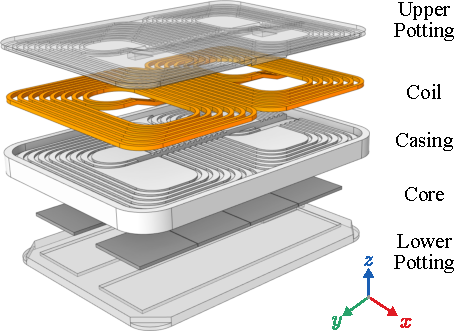
\includegraphics{figures/padstructure.pdf}
  \caption{Typical structure of IPT pad for EV charging}
  \label{fig:padstructure}
\end{figure}
\begin{figure}[t]
  \centering
  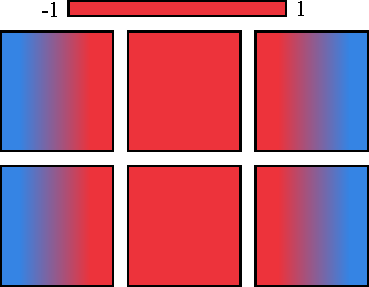
\includegraphics{figures/simulatedpottingpadstresses.pdf}
  \caption{FEA simulation of compressive stresses on ferrites during curing}
  \label{fig:pottingstresses}
\end{figure}

\section{Characterisation of Ferrite Under Stress}
Stress is a physical quantity that describes the forces acting on a material, simple uniaxial stress in the $z$ direction $\sigma_z$ can be calculated from, 
\begin{equation}
  \sigma_z = \frac{F_z}{A}
\end{equation}
Where $F_z$ is the compressive force acting in the $z$ direction and $A$ is the cross-sectional area normal to the $z$-axis. 
Although the major stresses on ferrite tiles in IPT are shear (forces act to push layers of the material co-planar to each other), this article considers the material under compressive loading to simplify the measurement setup. 
The von Mises equivalent stress is a scalar value that represents the effect of each of the individual stress components, principal and shear, the von Mises equivalent stress $\sigma_\text{eqv}$ is used in this article to allow for comparisons between the measured compressive stress and the predicted and measured shear stresses caused by the encapsulation material. 
By convention, compressive stress is negative and tensile stress is positive, however for simplicity, in this paper, compressive stress is considered positive unless the von Mises equivalent stress is used. 

\begin{comment}
\begin{equation}
  \sigma_\text{eqv} = \sqrt{
    \frac{1}{2} \left[
    \left( \sigma_{11} - \sigma_{22} \right) ^ 2 +
    \left( \sigma_{22} - \sigma_{33} \right) ^ 2 + 
    \left( \sigma_{33} - \sigma_{11} \right) ^ 2 \right] 
    + \left( \sigma_{12}^2 + \sigma_{23}^2 + \sigma_{31}^2 \right)
  }
\end{equation}
\end{comment}

A hydraulic press was used to apply a compressive force to the surface of toroid. 
However, in order to measure core loss in the hydraulic press, the toroid must be wound with two conductive windings. 
Conventional litz wire was eschewed since the sensitive strands would fail under significant compressive loading. 
Instead, a PCB was designed to form two robust windings which were than clamped to the toroid with M5 brass bolts. 
To avoid creating nonuniform pressure points in the toroid by apply pressure to the bolts, the top and bottom of the holder were potted with Electrolube UR5608. 
\cref{fig:compressionholder} shows an overview of the designed setup. 

\begin{figure}
  \centering
  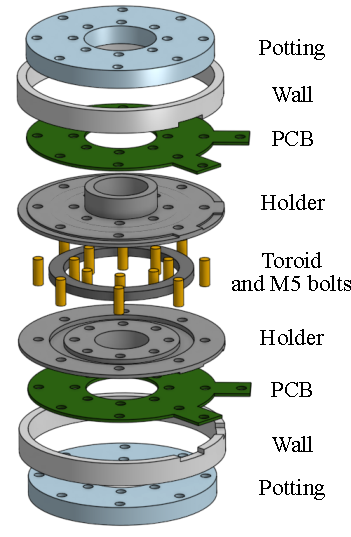
\includegraphics{figures/compressionholder.pdf}
  \caption{Exploded diagram of designed toroid compression setup}
  \label{fig:compressionholder}
\end{figure}

To verify the applied force was uniformly distributed across the toroid in the designed setup, a structural FEA simulation of the setup for each intended load was carried out. 
\cref{fig:holderfea} shows the predicted loads for the maximum required weight, designed to apply a \SI{120}{\mega\pascal} compressive stress to the ferrite toroid.
The equivalent stress distribution on the toroid is very uniform with a maximum difference across the surface of \SI{2}{\mega\pascal}. 

\begin{figure}
  \centering
  
\includegraphics[width=3.5in, height=2in]{figures/holderfea.pdf}
  \caption{FEA simulation of holder for \SI{96}{\kilo\newton} load}
  \label{fig:holderfea}
\end{figure}
\begin{table}
  \centering
  \caption{Toroid properties}
  \begin{tabular}{@{}llll@{}}
    \toprule
    Material & Manufacturer & $\alpha$ $\times 10^{-6}$ & $Y$ \\ \midrule
    N95 Ferrite & TDK & $10$ & \SI{119}{\giga\pascal} \\
    Nylon & TDK & $10$ & \SI{119}{\giga\pascal} \\
    FR4 PCB & TDK & $10$ & \SI{119}{\giga\pascal} \\
    UR5608 & TDK & $10$ & \SI{119}{\giga\pascal} \\
    PX900D & TDK & $10$ & \SI{119}{\giga\pascal} \\
    ER2223 & TDK & $10$ & \SI{119}{\giga\pascal} \\
    \bottomrule
  \end{tabular}
\end{table}

For each mechanical loading scenario, the core loss $P_\text{core}$ was then measured using a partial cancellation method which modifies the conventional two-winding method with a compensation capacitor $C_s$ in series to cancel the reactive voltage across the inductor under test $L_t$ \cite{houNewHighFrequencyCore2017}. 
The equivalent circuit of this method is shown in \cref{fig:partialcancellationcircuit}.
$C_s$ could be selected to completely cancel the reactive power in the system, but maintaining resonance for different operating conditions is challenging. 
Instead, a partial cancellation method defines a voltage cancellation factor $k_v$, the ratio of the cancelled reactive voltage to the total reactive voltage, to only `partially' cancel the reactive component of $L_t$. 
The core loss can then be found from measurements of the current flowing through the primary winding $i_L(t)$, the voltage on the secondary winding $v_2(t)$ and the voltage across the compensation capacitor $v_C(t)$ from, 
\begin{equation}
  P_\text{core} = f \int_0^T v_2(t)i_L(t)dt + \frac{f}{k_v} \int_0^T v_c(t)i_L(t) dt
\end{equation}
\begin{equation}
  P_\text{core}^{\prime} = f \int_0^T v_2(t)i_L^{\prime} (t)dt + \frac{f}{k_v} \int_0^T v_c(t)i_L^{\prime}(t) dt
\end{equation}
\begin{equation}
  k_v = \frac{\int_0^T v_c(t)i_L(t)dt - \int_0^T v_ci_L^\prime(t)dt}{\int_0^T v_2(t) i_L^\prime(t) dt - \int_0^T v_2(t) i_L(t) dt}
\end{equation}

\begin{figure}[t]
  \begin{subfigure}{\columnwidth}
    \centering
    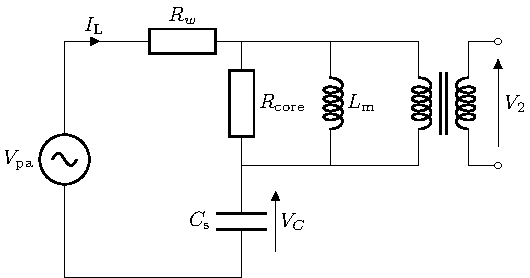
\includegraphics{figures/partialcancellationcircuit.pdf}
    \caption{}
    \label{fig:partialcancellationcircuit}
  \end{subfigure}
  \begin{subfigure}{\columnwidth}
    \centering
    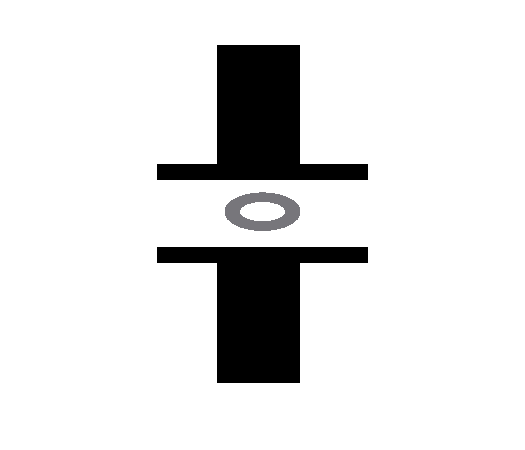
\includegraphics{figures/experimentalsetup.pdf}
    \caption{}
    \label{fig:experimentalsetup}
  \end{subfigure}
  \caption{(a) Equivalent circuit of the partial cancellation method, (b) Experimental setup for core loss measurement under compressive stress}
\end{figure}

\begin{figure}[t]
  \centering
  \begin{subfigure}{\columnwidth}
    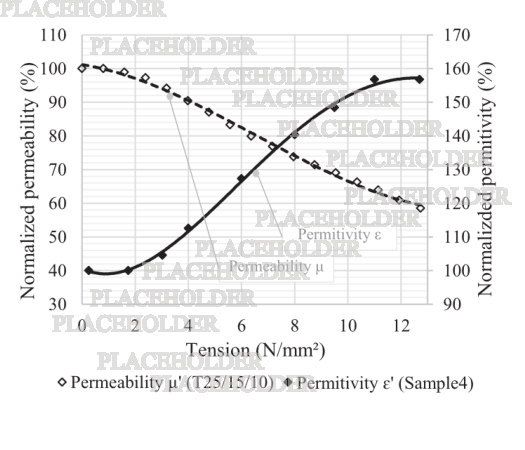
\includegraphics[width=3.5in, height=2in]{figures/changingBH.pdf}
    \caption{}
    \label{fig:changingBH}
  \end{subfigure}
  \begin{subfigure}{\columnwidth}
    \centering
    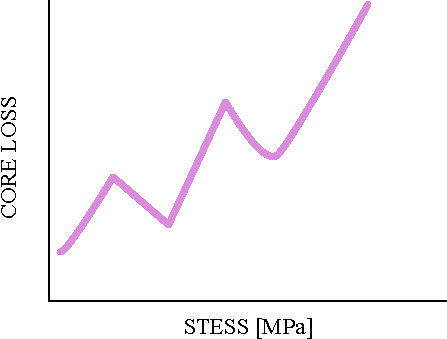
\includegraphics[width=3.5in, height=2in]{figures/coreloss.pdf}
    \caption{}
    \label{fig:coreloss}
  \end{subfigure}
  \caption{(a) $B$-$H$ curves of the TDK N95 ferrite toroid under several levels of compressive loading, (b) Core loss of TDK N95 ferrite toroid under several levels of compressive loading}
\end{figure}

\section{Verification of Core Loss Measurements}

This section presents two experiments which verify the measured results from the previous section. 
Firstly, three toroids of TDK N95 ferrite were potted with different encapsulation materials and the measured core loss compared to FEA simulations using the measured data. 
Finally, the core loss of a constructed Double D IPT pad is compared before and after potting, and the core loss after potting is predicted using the measured results. 

\subsection{Potted Toroid Measurement}

In order to verify the accuracy of the structural FEA simulations, three toroids of the same dimensions as described in the previous section were potted with different materials.
The potted toroids and the FEA predicted equivalent stress is shown in \cref{fig:pottedtoroids}.
The harder encapsulation materials show high residual stresses and hence higher core loss. 
However, the designer must trade off the desired mechanical behaviour of the encapsulation material and the effect of the encapsulation material on the system core losses. 

\begin{figure*}
  \centering
  \begin{subfigure}{\textwidth}
    \begin{subfigure}{0.3\textwidth}
      \centering
      
\includegraphics{figures/toroid.pdf}
      \caption{UR5608}
    \end{subfigure}~
    \begin{subfigure}{0.3\textwidth}
      \centering
      
\includegraphics{figures/toroid.pdf}
      \caption{PX900D}
    \end{subfigure}~
    \begin{subfigure}{0.3\textwidth}
      \centering
      
\includegraphics{figures/toroid.pdf}
      \caption{ER2223}
    \end{subfigure}

    \begin{subfigure}{0.3\textwidth}
      \centering
      
\includegraphics{figures/featoroid.pdf}
      \caption{}
    \end{subfigure}~
    \begin{subfigure}{0.3\textwidth}
      \centering
      
\includegraphics{figures/featoroid.pdf}
      \caption{}
    \end{subfigure}~
    \begin{subfigure}{0.3\textwidth}
      \centering
      
\includegraphics{figures/featoroid.pdf}
      \caption{}
    \end{subfigure}
  \end{subfigure}
  \caption{Experimental potted toroids and FEA structural simulations}
  \label{fig:pottedtoroids}
\end{figure*}

\begin{table}
  \centering
  \caption{Mechanical properties of relevant materials}
  \begin{tabular}{@{}llll@{}}
    \toprule
    Material & Manufacturer & $\alpha$ $\times 10^{-6}$ & $Y$ \\ \midrule
    N95 Ferrite & TDK & $10$ & \SI{119}{\giga\pascal} \\
    Nylon & TDK & $10$ & \SI{119}{\giga\pascal} \\
    FR4 PCB & TDK & $10$ & \SI{119}{\giga\pascal} \\
    UR5608 & TDK & $10$ & \SI{119}{\giga\pascal} \\
    PX900D & TDK & $10$ & \SI{119}{\giga\pascal} \\
    ER2223 & TDK & $10$ & \SI{119}{\giga\pascal} \\
    \bottomrule
  \end{tabular}
\end{table}

\subsection{Core Loss Prediction of Potted IPT Pad}
The core loss of a Double D IPT pad designed for \SI{11}{\kilo\watt} was measured using the stepped resonance method described in \cite{kalraPowerLossMeasurement2020}.
At rated current, the unpotted pad showed a total loss of \SI{0}{\watt}, with \SI{0}{\watt} of core loss.
When potted in two pours with UR5608, the total loss increased to \SI{0}{\watt} with \SI{0}{\watt} of core loss. 
\cref{fig:pottingstresses} shows an FEA simulation of the stress induced by this potting process. 
Use the predicted equivalent stress in the ferrites, the Steinmetz coefficients for each ferrite tile were adjusted accordingly and the core loss distribution shown in \cref{fig:padcoreloss} was predicted. 
The FEA simulation predicted a core loss of \SI{0}{\watt}, an error of \SI{0}{\percent}. 
\begin{figure}[t]
  %\includegraphics[width=3.5in, height=2in]{figures/padcoreloss}
  \includegraphics[width=3.5in, height=2in]{figures/pottingstresses}
  \caption{Predicted core loss distribution in DD pad with results of this article}
  \label{fig:padcoreloss}
\end{figure}

\section{Conclusion}

\section*{References}
\printbibliography[heading=none]


\end{document}
